Part of speech tagging is probably one the most common NLP tasks. The
task is to assign each word a grammatical category, \emph{i.e.} Noun,
Verb, Adjective, ... . In English, using the Penn Treebank (PTB)~\citep{pennTreeBank}, the current
state of the art for part of speech tagging is around 97\% for a
variety of methods \footnote{See ACL state of the art wiki}.

In the rest of this class we will use a subset of the PTB corpus, but
instead of using the original 45 tags we will use a reduced tag set of
12 tags, to make the algorithms faster for the
class. In this task, $\sent$ is a sentence and $\hseq$
is the sequence of possible PoS tags.

The first step is to load the pos corpus. We will start by loading
1000 sentences for training and 200 sentences both for development and
testing, and training the HMM model.
\begin{python}
In []: run readers/pos_corpus.py
In []: corpus = PostagCorpus()
In []: train_seq = corpus.read_sequence_list_conll("../data/train-02-21.conll",max_sent_len=15,max_nr_sent=1000)
unknown tag po
unknown tag pr
unknown tag wd
unknown tag pd
unknown tag wr
unknown tag sy
In []: test_seq = corpus.read_sequence_list_conll("../data/test-23.conll",max_sent_len=15,max_nr_sent=1000)
unknown tag pr
unknown tag po
unknown tag wr
unknown tag wd
unknown tag pd
unknown tag sy
In []: dev_seq = corpus.read_sequence_list_conll("../data/dev-22.conll",max_sent_len=15,max_nr_sent=1000)
unknown tag wd
unknown tag wr
unknown tag po
unknown tag pr
unknown tag pd
In []: corpus.add_sequence_list(train_seq) 
In []: run sequences/hmm.py
In []: hmm = HMM(corpus)
In []: hmm.train_supervised(train_seq)
In []: hmm.print_transition_matrix()
\end{python}

Ignore the warnings -- they are a consequence of our choice of using only a reduced set of 12 tags instead of the full set of POS tags.

%Note the warning ``Warning: invalid value encountered in divide`` due to the lack of smoothing. This is because we are trying to
%estimate the probability of words that were never seen during
%training, so the counts are zero and, when normalizing to get probabilities, we are trying to do 0/0. 

Look at the transition probabilities of the trained model, using the commands
\begin{python}
In []: import matplotlib.pyplot as plt
In []: hmm.transition_probs
\end{python}

 (see
Figure \ref{fig:transProbs}), and see if they match your intuition
about the English language (e.g. adjectives tend to come before nouns).

\begin{figure}
\centering
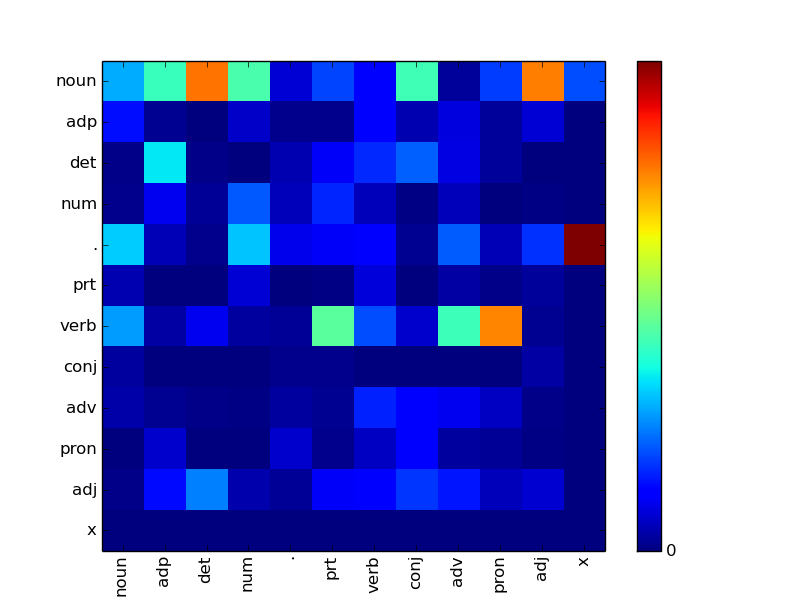
\includegraphics[scale=.5]{figs/sequences/transition_probs}
\caption{\label{fig:transProbs} Transition probabilities of the
trained model. Each column is previous state and row is current
state. Note the high probability of having Noun after Adjective, or of having Verb after Noun, as expected.}
\end{figure}

\begin{exercise}
Test the model using both posterior decoding and viterbi decoding on
both the train and test set, using the methods in class HMM:
\begin{python}
In []: viterbi_pred_train = hmm.viterbi_decode_corpus(train_seq.seq_list)
In []: posterior_pred_train = hmm.posterior_decode_corpus(train_seq.seq_list)
In []: eval_viterbi_train =   hmm.evaluate_corpus(train_seq.seq_list,viterbi_pred_train)
In []: eval_posterior_train = hmm.evaluate_corpus(train_seq.seq_list,posterior_pred_train)
In []: eval_viterbi_train
Out[]: 0.9811604369175269
In []: eval_posterior_train
Out[]: 0.9811604369175269

In []: viterbi_pred_test = hmm.viterbi_decode_corpus(test_seq.seq_list)
In []: posterior_pred_test = hmm.posterior_decode_corpus(test_seq.seq_list)
In []: eval_viterbi_test =   hmm.evaluate_corpus(test_seq.seq_list,viterbi_pred_test)
In []: eval_posterior_test = hmm.evaluate_corpus(test_seq.seq_list,posterior_pred_test)
In []: eval_viterbi_test
Out[]: 0.5224796989502872
In []: eval_posterior_test
Out[]: 0.3798772034066152


\end{python}

What do you observe? Remake the previous exercise but now train the HMM
using smoothing. Try different values and report the results on the
train and development set (1,0.1,0.001,0.0001). (Use function
\emph{pick\_best\_smoothing}).


\begin{python}
In []: hmm.pick_best_smoothing(train_seq,dev_seq,[0,0.1,0.01,1])
Smoothing 0.000000 --  Train Set Accuracy: Posterior Decode 0.981, Viterbi Decode: 0.981
sequences/hmm.py:214: RuntimeWarning: invalid value encountered in double_scalars
  posteriors[current_state,pos] = forward[current_state,pos]*backward[current_state,pos]/likelihood
Smoothing 0.000000 -- Test Set Accuracy: Posterior Decode 0.401, Viterbi Decode: 0.539
Smoothing 0.100000 --  Train Set Accuracy: Posterior Decode 0.969, Viterbi Decode: 0.965
Smoothing 0.100000 -- Test Set Accuracy: Posterior Decode 0.865, Viterbi Decode: 0.854
Smoothing 0.010000 --  Train Set Accuracy: Posterior Decode 0.981, Viterbi Decode: 0.980
Smoothing 0.010000 -- Test Set Accuracy: Posterior Decode 0.843, Viterbi Decode: 0.835
Smoothing 1.000000 --  Train Set Accuracy: Posterior Decode 0.884, Viterbi Decode: 0.878
Smoothing 1.000000 -- Test Set Accuracy: Posterior Decode 0.821, Viterbi Decode: 0.812
Out[]: 0.1
\end{python}

As before, the warnings are due to tags in the dev set which were not present in the train set -- just ignore them. Using the best smoothing value (0.1) evaluate the accuracy on the test set.

\begin{python}
In []: hmm.train_supervised(train_seq,smoothing=0.1)
In []: pred = hmm.viterbi_decode_corpus(test_seq.seq_list)
In []: eval_test = hmm.evaluate_corpus(test_seq.seq_list,pred)
In []: eval_test
Out[]: 0.8377896613190731
\end{python}

Perform some error analysis to understand were the errors are coming
from. You can start by visualizing the confusion matrix (true tags vs
predicted tags).

\begin{python}
In []: run sequences/confusion_matrix.py
In []: cm = build_confusion_matrix(test_seq.seq_list,pred,len(corpus.int_to_tag),hmm.nr_states)
In []: plot_confusion_bar_graph(cm,corpus.int_to_tag,xrange(hmm.nr_states),tag_colors)
In[]: plt.show()
\end{python}

\begin{figure}
\centering
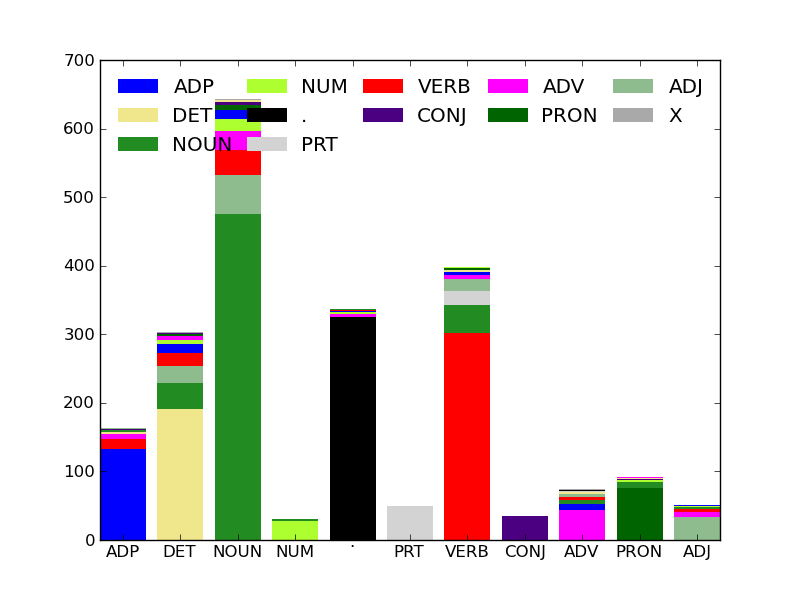
\includegraphics[scale=.5]{figs/sequences/cm_sup.png}
\caption{\label{fig:cm_uns} Confusion Matrix for the previous
  example. Predict tags are columns and the true tags corresponds to
  the constituents of each column.}
\end{figure}

%Another option to look at is to the error for words with different
%number of occurrences, rare words vs common words.
\end{exercise}


%\begin{exercise}
%Implement a function that produces the accuracy for rare words vs
%common words. Use you own definition of rare word.
%
%Can you come up with other error analysis methods? Which?
%
%\end{exercise}

\begin{exercise}
So far we have only worked with a limited dataset of 1000 words. Try increasing the number of sentences to 10000. What do you observe?

\end{exercise}
